\chapter{Discussion}
\section{Solutions comparison}

\begin{table}[h]
    \centering
    \begin{tabular}{lcccc}
        \toprule
        \textbf{Model name} & \textbf{Accuracy} & \textbf{Precision} & \textbf{Recall} & \textbf{F1 score} \\ 
        \midrule
        EPDB & 99.36 & 98.87 & 100.00 & 99.43 \\
        PDGAN & 97.58 & 98.02 & 97.27 & 97.64 \\
        PhishingTransformer & 98.90 & 98.80 & 99.00 & 98.80 \\
        \bottomrule
    \end{tabular}
    \caption{Solutions Comparison}
    \label{tab:solutions_comparison}
\end{table}

\textbf{EPDB} achieves the highest performance metrics, but it's important to note that this result is based on a relatively small dataset of 11,055 records. The exceptional results could indicate that the model is well-tuned for the specific dataset but might require further validation on larger, more diverse datasets to ensure its robustness in broader applications.

\textbf{PhishingTransformer} also shows strong performance with a dataset of 100,000 records. This model strikes a good balance between precision and recall, demonstrating its effectiveness on a moderately sized dataset. Its near-perfect metrics suggest that it generalizes well, even with a significantly larger dataset than EPDB's.

\textbf{PDGAN}, despite using a much larger dataset of 2.3 million records, has slightly lower performance metrics. This could suggest that while PDGAN is effective at processing large-scale data and maintaining high precision, it faces challenges in achieving the same level of recall and overall accuracy as the other models. However, its ability to handle such a large dataset indicates its scalability and potential for real-world applications where large volumes of data are common.

\section{Considerations}
Qualitatively, the datasets used by the authors of the three models differ from each other, but they mostly come from the same sources, so they can be assumed to be fairly similar. However, quantitatively, they cannot be considered similar since the \textbf{EPDB} dataset is one-tenth the size of the \textbf{PhishingTransformer} dataset, which is 20 times smaller than the \textbf{PDGAN} dataset. Therefore, it is difficult to determine the absolute best model.

Regarding the \textbf{EPDB} model, we have information on its performance in terms of execution speed 4 seconds for the Random Forest model. The other deep learning solutions are undoubtedly more complex and require more time both during training and inference.

The authors of \textbf{EPDB} and \textbf{PhishingTransformer} use the k-fold cross-validation technique to obtain more reliable and stable statistical estimates of model performance. However, the authors of \textbf{PhishingTransformer} use this technique to allow the model to learn from the validation set as well, as explained in their paper in section 4.5: \textit{"Therefore, it ensures that every data point contributes to training and validation, maximizing the utilization of our dataset."} This approach, however, does not utilize k-fold cross-validation but rather trains the same model five times on the entire training dataset (80\% of the total). This is also evident from the graph provided by the authors, where the model's performance, instead of varying slightly, increases sharply after the first fold and reaches perfection by the fifth fold, likely resulting in overfitting.

\begin{figure}[htp]
    \centering
    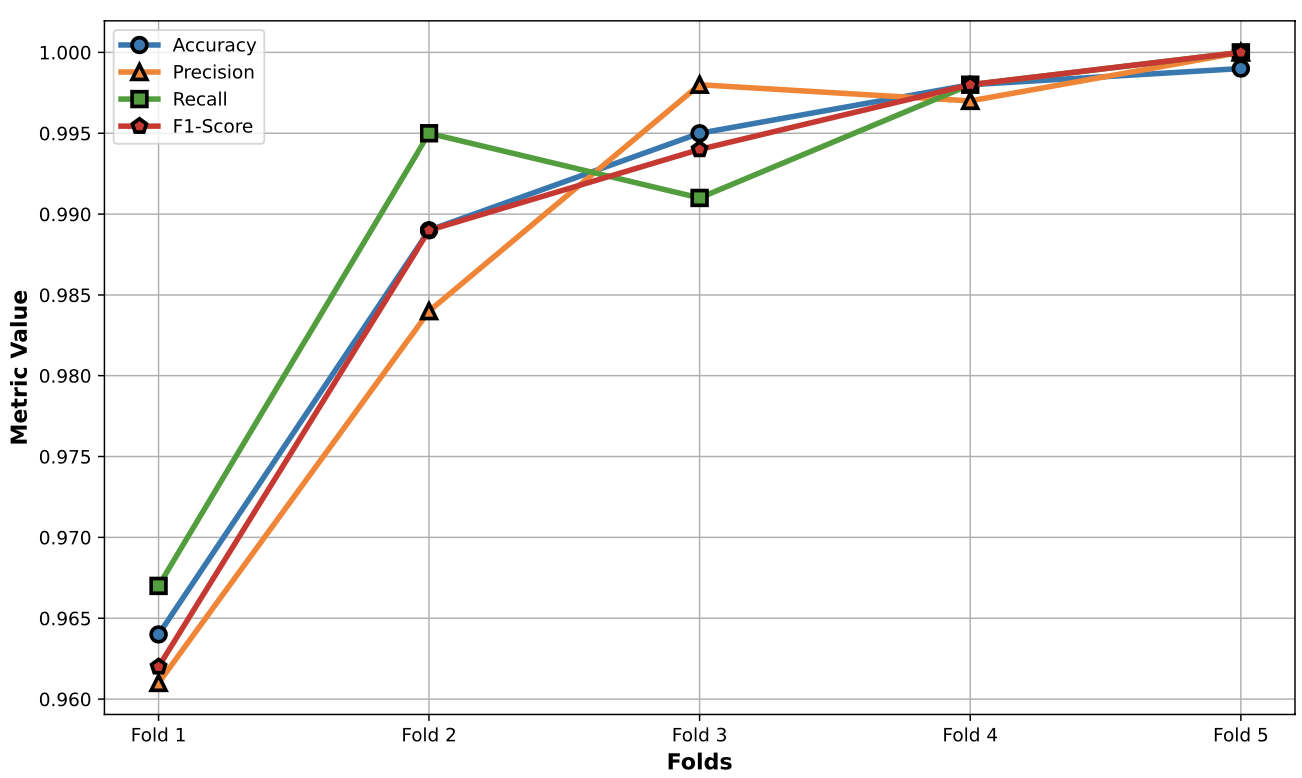
\includegraphics[width=0.8\linewidth]{images/K-fold errror.png}
    \caption{Five-fold cross validation}
    \label{fig:Five-fold cross validation}
\end{figure}
The authors of \textbf{DPGAN} created a model that not only can distinguish between a safe and an unsafe website but also is capable of generating new URLs. They use the generator to create 50,000 synthetic URLs and add them to the dataset to improve the model's performance. This technique is not universally accepted among researchers because, while it offers the advantage of data augmentation and helps address data scarcity, it also has the drawback of potentially leading to overfitting on synthetic data. The discriminator might become overly reliant on synthetic data, reducing its effectiveness on real data. However, in this case, considering that the synthetic data accounts for only 1/40th of the total dataset, the model's improvement can be accepted without significant concern for overfitting on synthetic data.

Regarding hyperparameter optimization, \textbf{EPDB} uses GridSearchCV, ensuring that the best possible results are obtained. Similarly, \textbf{PDGAN} involved varying hyperparameters to choose the optimal solution. On the other hand, for \textbf{PhishingTransformer}, assumptions were made regarding the length of URLs and the number of embedded URLs, while the other CNN hyperparameters were left at their default settings.

However, \textbf{PhishingTransformer} introduces an interesting hybrid-based solution compared to the other two URL-based solutions, which helps prevent phishing attacks through "embedding malicious code in legitimate content."

\section{Conclusion and future improvements}
The authors of PDGAN and PhishingTransformer propose an innovative AI model, which uses a CNN to extract URL features and an LSTM or Encoder to understand the relationships between URL characters. In contrast, the authors of EPDB present a complete system, specifically a secure browser. With some modifications, it might be possible to replace or integrate the ML prediction model with one of the deep learning techniques proposed by the other authors.

It could also be interesting to explore continuous or federated learning techniques to keep the models continuously updated without the need to retrain the entire model, which, especially in the case of Deep Learning  techniques, becomes particularly time-consuming.

As potential improvements, increasing the dataset for EPDB is essential, as it is too small, and similarly for PhishingTransformer, which, although ten times larger than EPDB’s, still remains a deep learning technique that requires much more data to effectively learn the network weights. Additionally, a model could be developed that incorporates predictions from all three models and makes a decision based on a weighted average.